\chapter{Background}
This chapter describes the hardware and software tools used in the project.

\section{Hardware}
\subsection{Particle Photon}
The Particle Photon is a tiny board (36.58mm $\times$ 20.32mm $\times$ 4.32mm in our configuration, weighing in at 5 grams) specifically designed for IoT\footnote{Internet of Things: a system of typically embedded devices that connects to the Internet and to each other, without requiring human-to-human or human-to-computer interaction \cite{WikipediaIoT}. There's still no baseline or standard definition, which is why IEEE is asking for suggestions to the community to provide it \cite{IEEEIoT}.} projects \cite{ParticlePhoton}, based on a relatively powerful but power efficient microcontroller of the STM32 ARM Cortex M3 family, with integrated Wi-Fi and the ability to interface itself with cloud services offered by Particle.\\
Unfortunately, the integrated Wi-Fi module was not powerful enough to ensure a reliable connection in the tested scenarios, causing frequent disconnections. An Airgain's IPEX antenna, easily pluggable to the Photon through a U.FL connector, has allowed to achieve a more stable connection.
The code deployment can be performed seamlessly through a web-based IDE, that compiles and flashes the code to the selected device OTA (Over-The-Air). It is also possible to control the real-time device's status through a web-based too console, that allows to flash the firmware to a specific version (downgrades are trickier than upgrades, especially OTA), and displays graphs for data such Wi-Fi's signal strength and quality, round trip time and memory usage.

\begin{center}
	\begin{figure}[ht!]
		\makebox[\textwidth]{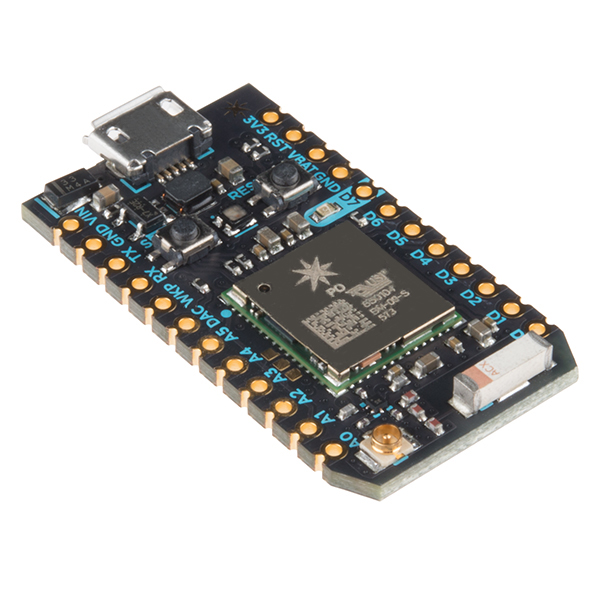
\includegraphics[width=0.3\paperwidth]{img/photon.jpg}}
		\caption{Particle Photon \cite{Photon}.}
	\end{figure}
\end{center}

\subsection{Sensors}
The SparkFun's sensor stick used in the project is a 9DoF (Degrees of Freedom) MARG (Magnetic, Angular Rate and Gravity) MEMS (Micro-Electro-Mechanical Systems) sensor. Its inertial module is the STMicroelectronics's LSM9DS1 integrated circuit, that features a digital linear acceleration sensor a digital angular rate sensor and a digital magnetic sensor: each one can make measurements from $x$, $y$ and $z$ axes, and that's where the 9 degrees of freedom came from. The stick has been connected to the Photon through the I$^2$C serial bus interface. Its compact size and power efficiency make it ideal for embedded systems \cite{SensorDatasheet}.
\begin{center}
	\begin{figure}[ht!]
		\makebox[\textwidth]{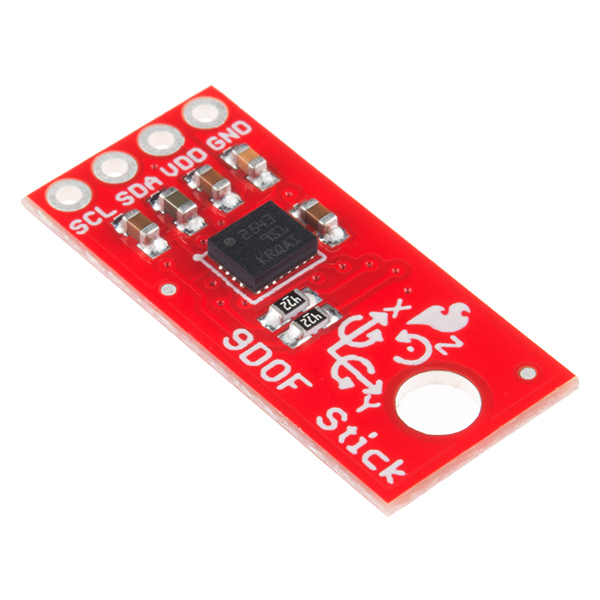
\includegraphics[width=0.3\paperwidth]{img/imu.jpg}}
		\caption{SparkFun Sensor Stick \cite{IMU}.}
	\end{figure}
\end{center}

\section{Software}

\subsection{Node.js}
Node.js is an open-source asynchronous event-driven JavaScript runtime environment that executes code outside of a browser, built on Google Chrome's V8 JavaScript engine \cite{Node.js}.\\
To put it simply, a synchronous execution environment needs to wait to one task to finish before moving to another; asynchronous execution, on the contrary, allows to move to another task before the previous one finishes. In a network context (typically I/O bound), for a single-threaded software (like Node.js) a asynchronous (non-blocking) I/O (input/output) method allows to register the clients' requests, wait for until the reply is available, and then call the related callback, allowing faster replies to the clients, compared to synchronous (blocking) I/O.

\subsection{Express.js}
Express.js, or simply Express, is a minimalist, open-source web framework for Node.js, designed for building web applications and APIs \cite{Express.js}. Its main feature is the routing mechanism: it allows to specify a callback function called when the application receives a request to the specified route and HTTP method. For example, using an Express \texttt{app} object, \texttt{app.get()} would handle GET requests, \texttt{app.post()} would handle POST ones, and so on.

\subsection{Three.js}
Three.js is a JavaScript library for creating animated 3D graphics in a web browser. Three.js uses WebGL (and simplifies its API) for creating GPU-accelerated 3D animations within web browsers without relying on proprietary plugins; in fact, Three.js is fully open-source.

\subsection{MQTT}
MQTT (Message Queue Telemetry Transport) is a machine-to-machine (M2M)/"Internet of Things" connectivity protocol \cite{MQTT}. MQTT was designed as an extremely lightweight publish/subscribe messaging transport, and can be supported by any network protocol that provides ordered, lossless and bi-directional connections \cite{MQTTDoc} (typically TCP/IP).\\
The MQTT protocol defines two types of network entities: a message broker (Mosca in the project) and a number of clients. An MQTT broker is a server that receives all messages from the clients and then routes the messages to the appropriate destination clients \cite{KnowMQTT}. An MQTT client is any device that runs an MQTT library and connects to an MQTT broker over a network \cite{ClientBroker}.\\
Information is organized in a hierarchy of topics. When a publisher has a new item of data to distribute, it sends a control message with the data to the connected broker. The broker then distributes the information to any clients that have subscribed to that topic. The publisher does not need to have any data on the number or locations of subscribers, and subscribers in turn do not have to be configured with any data about the publishers.

\subsection{MongoDB}
MongoDB is a general purpose, document-based, distributed database \cite{MongoDB}. Classified as a NoSQL database, stores documents in a JSON-like format with schema. MongoDB belongs to the category of document-oriented databases: the smallest unit of storage is a document; documents are stored in a collection, which in turn make up a database. Document are analogous to rows in a SQL table, but with one big difference: not every document needs to have the same structure. Another feature of MongoDB is that fields in a document can contain arrays and or sub-documents (sometimes called nested or embedded documents).\\
MongoDB stores data records as BSON documents. BSON is a binary representation of JSON documents, though it contains more data types than JSON \cite{BSONSpec}.

\subsection{TensorFlow}
\dots

\section{Rotation formalisms in three dimensions}
\dots

\section{Filters}
Motion representation can be obtained through accelerometer reading within the $x$, $y$ and $z$ axes, that make up an acceleration vector.\\
MEMS sensors are known to be very noisy, especially when working at high reading frequencies \cite[7]{Mat08}, and the noise is of a specific type, the Additive White\footnote{White noise is a random signal with constant amplitude across the whole frequency spectrum.} Gaussian\footnote{Noise having a probability density function equal to that of the normal distribution, which is also known as the Gaussian distribution \cite{WikipediaGaussianNoise}.} Noise (AWGN) \cite{Yas03}. An effective way to remove AWGN is to use the Kalman filter, because of its characteristics \cite{Ko07, Sär15}.

\subsection{Kalman filter}
Kalman filtering, also known as linear quadratic estimation (LQE), is an efficient recursive algorithm that uses a series of measurements observed over time, containing statistical noise and other inaccuracies, and produces estimates of unknown variables (the internal state of a linear dynamic system\footnote{Linear dynamic systems are systems in which its evolution is described by a linear function and hence satisfies the superposition principle.}) that tend to be more precise than those based on a single measurement alone, by using Bayesian inference and estimating a joint probability distribution over the variables for each timeframe.\\
Using a Kalman filter does not assume that the errors are Gaussian \cite{Kal60}. However, the filter yields the exact conditional probability estimate in the special case that all errors are Gaussian \cite{WikipediaKalman}.\\
Kalman filter is most often conceptualized as two distinct phases:

\begin{enumerate}
	\item time updating: prediction phase, where the previous timesteps are used to predict the current one's state (\textit{a priori} state estimate);
	\item measure update: observation phase, where the prediction is combined with the current observation information to refine the state estimate (\textit{a posteriori} state estimate).
\end{enumerate}

The Kalman filter has numerous applications in technology, like navigation and control of vehicles, particularly aircraft, spacecraft and dynamically positioned ships \cite{WikipediaKalman}.

\subsection{Madgwick filter} \label{Madgwick filter}
\dots

\section{Neural networks}
\dots
